\documentclass[tikz,border=3pt]{standalone}
\usepackage{xcolor}
\usetikzlibrary{arrows.meta,calc,decorations.pathreplacing}

% Shared with Figs. 1--2.
\definecolor{ink}{HTML}{24343D}
\definecolor{muted}{HTML}{657985}
\definecolor{environment}{HTML}{D9DEE3}
\definecolor{candidate}{HTML}{B5C1C8}
\definecolor{topology}{HTML}{657985}
\definecolor{depth}{HTML}{3973B7}
\definecolor{selected}{HTML}{007C83}
\definecolor{riskhigh}{HTML}{D14E46}
\definecolor{scorelow}{HTML}{EDF3F0}
\definecolor{scoremid}{HTML}{D9AD3D}
\definecolor{mission}{HTML}{C43C39}
\definecolor{frontier}{HTML}{E28A17}
\definecolor{localgoal}{HTML}{B64E8A}

\begin{document}
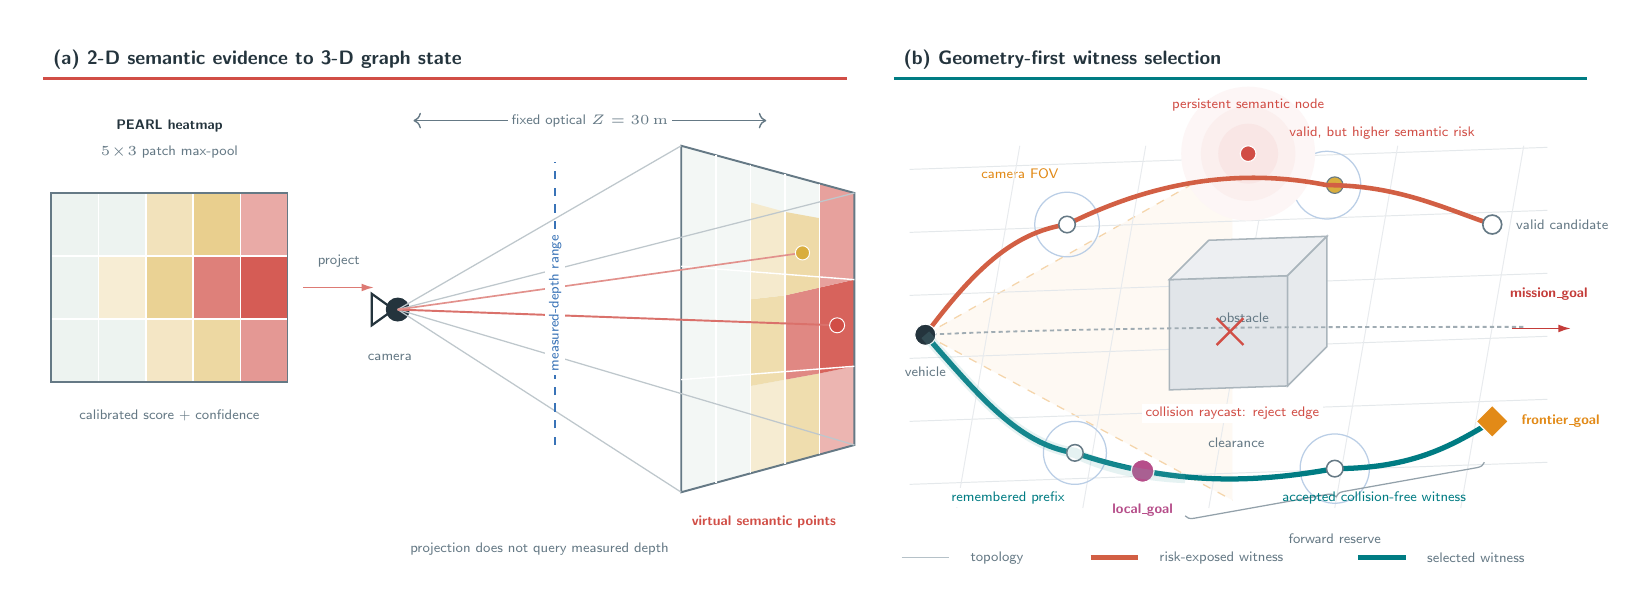
\begin{tikzpicture}[
  x=1mm,y=1mm,font=\sffamily,
  heading/.style={font=\sffamily\bfseries\fontsize{7.0}{8.0}\selectfont,text=ink},
  label/.style={font=\sffamily\bfseries\fontsize{5.0}{5.8}\selectfont,text=ink,align=center},
  note/.style={font=\sffamily\fontsize{4.3}{5.1}\selectfont,text=muted,align=center},
  tinylabel/.style={font=\sffamily\fontsize{3.9}{4.6}\selectfont,text=muted,align=center},
  flow/.style={-{Latex[length=1.6mm,width=1.0mm]},line width=.7pt},
  graphedge/.style={draw=candidate,line width=.65pt},
  selectededge/.style={draw=selected,line width=1.9pt},
  riskyedge/.style={draw=riskhigh!82!scoremid,line width=1.65pt}
]

% Make raster export and inclusion in the paper unambiguously white.
\fill[white] (-2,-2) rectangle (198,68);

% (a) Every pooled image patch owns a camera ray and a point on the fixed-Z plane.
\node[heading,anchor=west] at (0,64) {(a) 2-D semantic evidence to 3-D graph state};
\draw[riskhigh,line width=1.05pt] (0,61.5)--(102,61.5);

\node[label] at (16,55.5) {PEARL heatmap};
\node[note] at (16,52.2) {$5\!\times\!3$ patch max-pool};
\filldraw[fill=scorelow,draw=topology,line width=.65pt] (1,23) rectangle (31,47);
\foreach \x/\y/\c in {
  1/39/scorelow,7/39/scorelow,13/39/scoremid!35,19/39/scoremid!58,25/39/riskhigh!48,
  1/31/scorelow,7/31/scoremid!22,13/31/scoremid!55,19/31/riskhigh!72,25/31/riskhigh!92,
  1/23/scorelow,7/23/scorelow,13/23/scoremid!30,19/23/scoremid!48,25/23/riskhigh!58}
  {\fill[\c] (\x,\y) rectangle ++(6,8);}
\foreach \x in {7,13,19,25}{\draw[white,line width=.55pt] (\x,23)--(\x,47);}
\foreach \y in {31,39}{\draw[white,line width=.55pt] (1,\y)--(31,\y);}
\draw[topology,line width=.65pt] (1,23) rectangle (31,47);
\node[tinylabel,anchor=north] at (16,20.7) {calibrated score + confidence};

\draw[flow,draw=riskhigh!75] (33,35)--(42,35);
\node[tinylabel,fill=white,inner sep=.4mm] at (37.5,38.3) {project};
\filldraw[fill=ink,draw=ink] (45,32.2) circle (1.45mm);
\draw[ink,line width=.8pt] (41.7,30.2)--(44.5,32.2)--(41.7,34.2)--cycle;
\node[note,anchor=north] at (44,27.8) {camera};

% Fixed optical-Z plane in perspective; colors preserve the patch correspondence.
\fill[scorelow!65] (81,9)--(103,15)--(103,47)--(81,53)--cycle;
\fill[scoremid!23] (89.8,11.4)--(94.2,12.6)--(94.2,23.3)--(89.8,22.5)--cycle;
\fill[scoremid!42] (94.2,12.6)--(98.6,13.8)--(98.6,24.1)--(94.2,23.3)--cycle;
\fill[riskhigh!42] (98.6,13.8)--(103,15)--(103,25)--(98.6,24.1)--cycle;
\fill[scoremid!42] (89.8,22.5)--(94.2,23.3)--(94.2,34.0)--(89.8,33.5)--cycle;
\fill[riskhigh!67] (94.2,23.3)--(98.6,24.1)--(98.6,35.0)--(94.2,34.0)--cycle;
\fill[riskhigh!88] (98.6,24.1)--(103,25)--(103,36)--(98.6,35.0)--cycle;
\fill[scoremid!26] (89.8,33.5)--(94.2,34.0)--(94.2,44.6)--(89.8,45.8)--cycle;
\fill[scoremid!45] (94.2,34.0)--(98.6,35.0)--(98.6,43.8)--(94.2,44.6)--cycle;
\fill[riskhigh!53] (98.6,35.0)--(103,36)--(103,47)--(98.6,48.2)--cycle;
\draw[topology,line width=.7pt] (81,9)--(103,15)--(103,47)--(81,53)--cycle;
\foreach \xa/\ya/\xb/\yb in {85.4/10.2/85.4/51.8,89.8/11.4/89.8/50.6,
  94.2/12.6/94.2/49.4,98.6/13.8/98.6/48.2}
  {\draw[white,line width=.5pt] (\xa,\ya)--(\xb,\yb);}
\draw[white,line width=.5pt] (81,23.3)--(103,25);
\draw[white,line width=.5pt] (81,37.7)--(103,36);

\draw[topology!42,line width=.45pt] (45,32.2)--(81,9);
\draw[topology!42,line width=.45pt] (45,32.2)--(81,53);
\draw[topology!42,line width=.45pt] (45,32.2)--(103,15);
\draw[topology!42,line width=.45pt] (45,32.2)--(103,47);
\draw[riskhigh!80,line width=.7pt] (45,32.2)--(100.8,30.2);
\draw[riskhigh!62,line width=.6pt] (45,32.2)--(96.4,39.4);
\filldraw[fill=riskhigh,draw=white,line width=.35pt] (100.8,30.2) circle (.95mm);
\filldraw[fill=scoremid,draw=white,line width=.35pt] (96.4,39.4) circle (.9mm);

% Deliberately distinguish virtual semantic projection from measured depth.
\draw[depth,dashed,line width=.55pt] (65,15)--(65,51);
\node[tinylabel,text=depth,rotate=90,fill=white,inner sep=.5mm] at (65,33)
  {measured-depth range};
\draw[<->,topology,line width=.5pt] (47,56.2)--(91.8,56.2);
\node[note,fill=white,inner sep=.5mm] at (69.4,56.2) {fixed optical $Z=30\,\mathrm{m}$};
\node[label,text=riskhigh] at (91.5,5.2) {virtual semantic points};
\node[note] at (63,1.8) {projection does not query measured depth};

% (b) Projected nodes rank only the witnesses that pass physical validation.
\node[heading,anchor=west] at (108,64) {(b) Geometry-first witness selection};
\draw[selected,line width=1.05pt] (108,61.5)--(196,61.5);

\coordinate (start) at (112,29);
\fill[frontier!5] (start)--(151,51)--(151,8)--cycle;
\draw[frontier!36,dashed,line width=.45pt] (start)--(151,51) (start)--(151,8);
\node[tinylabel,text=frontier] at (124,49.5) {camera FOV};

\foreach \y in {10,18,26,34,42,50}{
  \draw[environment!70,line width=.35pt] (110,\y)--(191,\y+2.8);
}
\foreach \x in {116,132,148,164,180}{
  \draw[environment!60,line width=.35pt] (\x,7)--(\x+8,53);
}

% Solid 3-D obstacle.
\filldraw[fill=environment!78,draw=topology!55,line width=.55pt]
  (143,22)--(158,22.5)--(158,36.5)--(143,36)--cycle;
\filldraw[fill=environment!48,draw=topology!55,line width=.55pt]
  (143,36)--(148,41)--(163,41.5)--(158,36.5)--cycle;
\filldraw[fill=environment!63,draw=topology!55,line width=.55pt]
  (158,22.5)--(163,27.5)--(163,41.5)--(158,36.5)--cycle;
\node[tinylabel,text=topology] at (152.5,31.2) {obstacle};

% Direct connection fails the one-shot collision raycast.
\draw[topology!62,dashed,dash pattern=on 1.5pt off 1.15pt,line width=.65pt]
  (start)..controls(133,30)and(164,30)..(188,30);
\draw[riskhigh,line width=.85pt] (149.0,27.7)--(152.4,31.1)
  (149.0,31.1)--(152.4,27.7);
\node[tinylabel,text=riskhigh,fill=white,inner sep=.45mm] at (151,19.0)
  {collision raycast: reject edge};

\coordinate (u1) at (130,43);
\coordinate (u2) at (163,48);
\coordinate (ut) at (184,43);
\coordinate (l1) at (131,14);
\coordinate (l2) at (164,12);
\coordinate (lt) at (184,18);
\draw[graphedge] (start)..controls(118,37)and(123,42)..(u1)
  ..controls(142,49)and(153,50)..(u2)
  ..controls(172,48)and(178,45)..(ut);
\draw[graphedge] (start)..controls(119,21)and(124,15)..(l1)
  ..controls(143,10)and(153,10)..(l2)
  ..controls(174,12)and(179,15)..(lt);

% Bubble radii expose clearance validation in the scene.
\foreach \p/\r in {u1/4.1,u2/4.3,l1/4.0,l2/4.4}{
  \draw[depth!35,line width=.45pt] (\p) circle (\r mm);
}

% Persistent semantic node and continuous witness field.
\fill[riskhigh!5]  (153,52) circle (8.5mm);
\fill[riskhigh!9]  (153,52) circle (6.0mm);
\fill[riskhigh!14] (153,52) circle (3.8mm);
\filldraw[fill=riskhigh,draw=white,line width=.4pt] (153,52) circle (1.0mm);
\filldraw[fill=scoremid,draw=topology,line width=.4pt] (164,48) circle (1.05mm);
\node[tinylabel,text=riskhigh,anchor=south] at (153,56.2) {persistent semantic node};

\draw[riskyedge] (start)..controls(118,37)and(123,42)..(u1)
  ..controls(142,49)and(153,50)..(u2)
  ..controls(172,48)and(178,45)..(ut);
\draw[selectededge] (start)..controls(119,21)and(124,15)..(l1)
  ..controls(143,10)and(153,10)..(l2)
  ..controls(174,12)and(179,15)..(lt);

\foreach \p in {u1,l1,l2}{
  \filldraw[fill=white,draw=topology,line width=.55pt] (\p) circle (1.05mm);
}
\filldraw[fill=ink,draw=white,line width=.4pt] (start) circle (1.35mm);
\node[tinylabel,anchor=north] at (112,26.2) {vehicle};

\filldraw[fill=white,draw=topology,line width=.6pt] (ut) circle (1.2mm);
\node[tinylabel,anchor=west] at (185.8,43) {valid candidate};
\filldraw[fill=frontier,draw=white,line width=.45pt,rotate around={45:(lt)}]
  ($(lt)+(-1.45,-1.45)$) rectangle ($(lt)+(1.45,1.45)$);
\node[label,text=frontier,anchor=west] at (186.5,18) {frontier\_goal};

\filldraw[fill=localgoal,draw=white,line width=.45pt] (139.6,11.7) circle (1.45mm);
\node[label,text=localgoal,anchor=north] at (139.6,8.7) {local\_goal};
\draw[flow,draw=mission,line width=.65pt] (186.5,29.8)--(194,29.8);
\node[label,text=mission,anchor=south] at (191.2,32.1) {mission\_goal};

% Continuity and reserve remain visible without a detached objective formula.
\draw[selected!55,line width=3.7pt,opacity=.18]
  (start)..controls(119,21)and(124,15)..(l1)..controls(135,12)and(140,11)..(145,10.8);
\node[tinylabel,text=selected,fill=white,inner sep=.4mm] at (122.5,8.3)
  {remembered prefix};
\draw[decorate,decoration={brace,mirror,amplitude=1mm},topology!70,line width=.45pt]
  (145,6.0)--(183,12.8);
\node[tinylabel,anchor=north] at (164,5.0) {forward reserve};

\node[note,text=riskhigh] at (170,54.6) {valid, but higher semantic risk};
\node[note,text=selected] at (169,8.2) {accepted collision-free witness};
\node[tinylabel,text=topology] at (151.5,15.3) {clearance};

\draw[graphedge] (109,0.7)--(115,0.7);
\node[tinylabel,anchor=west] at (116.5,.7) {topology};
\draw[riskyedge] (133,0.7)--(139,0.7);
\node[tinylabel,anchor=west] at (140.5,.7) {risk-exposed witness};
\draw[selectededge] (167,0.7)--(173,0.7);
\node[tinylabel,anchor=west] at (174.5,.7) {selected witness};

\end{tikzpicture}
\end{document}
